\section{Системы управления: ELRS, FrSky и другие}

\subsection{Из чего состоит радиоуправление}
\begin{itemize}
\item \term{Пульт} (аппаратура, «радио») — стики, тумблеры, экран. Прошивка — обычно \textbf{EdgeTX} (открытая, наследник OpenTX). Модели: RadioMaster TX16S, Boxer, Zorro, Pocket; FrSky Taranis; TBS Tango 2; Jumper.
\item \term{Передающий модуль} (TX) — встроенный в пульт или внешний в отсек \textbf{JR} (большой) / \textbf{Nano} (Lite).
\item \term{Приёмник} (RX) на борту — связан с ПК по CRSF/SBUS/IBUS.
\item \term{Привязка} (bind) — пара «передатчик–приёмник» запоминают друг друга, чтобы не реагировать на чужие пульты.
\item \term{FHSS} — псевдослучайная перестройка частоты десятки–сотни раз в секунду: устойчивость к помехам и совместная работа многих пилотов.
\item \term{Failsafe} — поведение при потере связи: отключить моторы (drop), удерживать последние значения (hold) или возврат домой (RTH, GPS Rescue).
\item \term{RSSI} — уровень сигнала (дБм); \term{LQ} (Link Quality) — процент успешно принятых пакетов. LQ важнее RSSI.
\end{itemize}

\begin{figure}[H]\centering
\begin{minipage}[b]{0.30\linewidth}\centering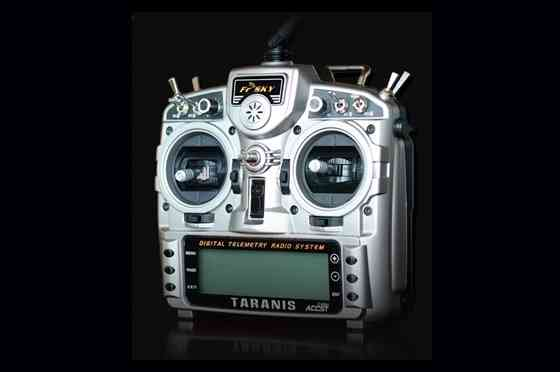
\includegraphics[width=\linewidth]{img/taranis.jpg}\\{\small FrSky Taranis}\end{minipage}\hfill
\begin{minipage}[b]{0.34\linewidth}\centering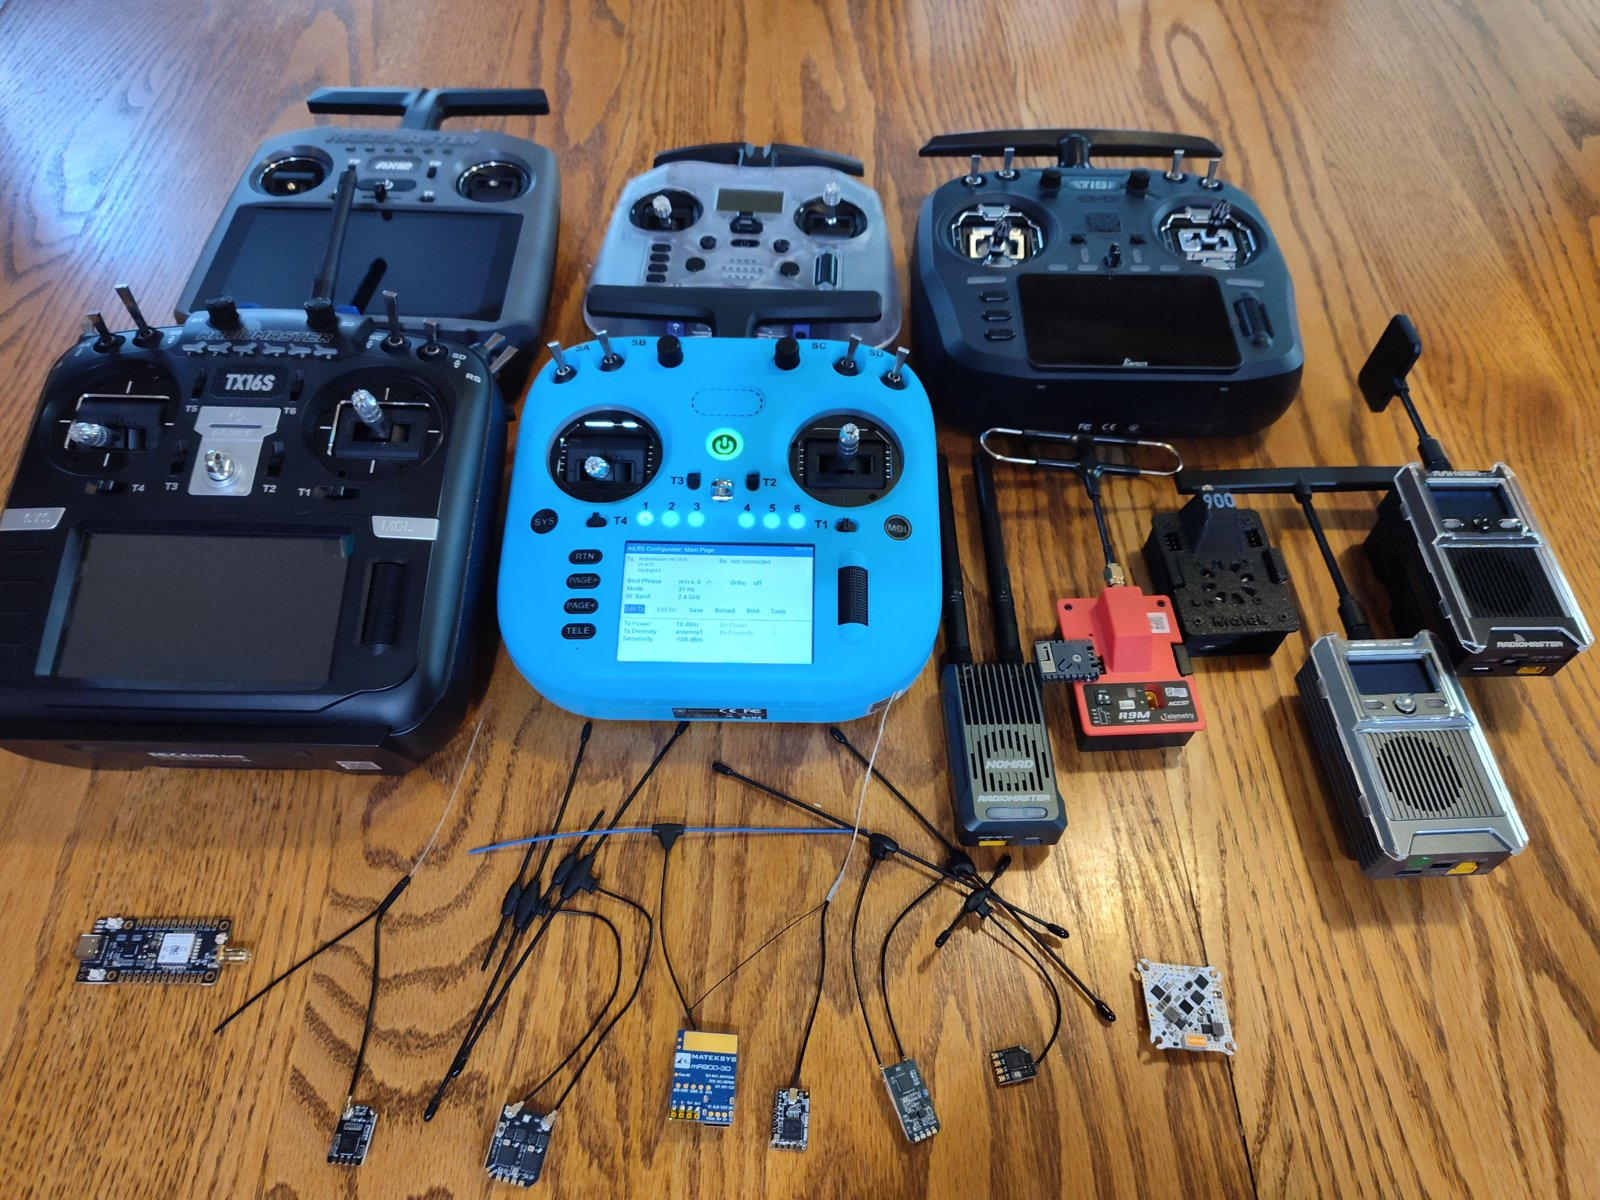
\includegraphics[width=\linewidth]{img/mlrs.jpg}\\{\small Пульты и модули на EdgeTX}\end{minipage}\hfill
\begin{minipage}[b]{0.30\linewidth}\centering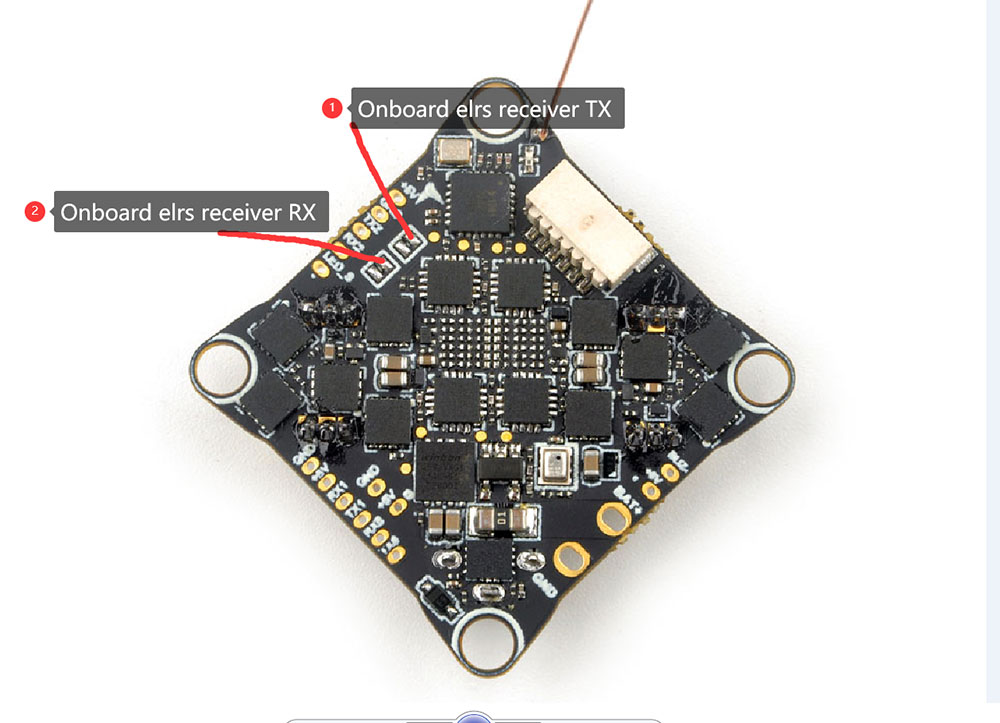
\includegraphics[width=\linewidth]{img/elrs-ext.jpg}\\{\small Приёмник ELRS на полётном контроллере}\end{minipage}
\caption{Аппаратура управления и приёмники {\color{gray}\scriptsize(фото: ArduPilot Wiki)}}
\end{figure}

\subsection{ExpressLRS (ELRS)}
\begin{itemize}
\item \textbf{Открытый} (open source) проект, появился в 2020 г. Сейчас — самый популярный RC-линк в FPV. Дешёвое железо многих производителей (RadioMaster, BetaFPV, HappyModel\ldots).
\item Радиочипы Semtech: \textbf{SX1280} (\SI{2.4}{\giga\hertz}), \textbf{SX1276} (\SIrange{868}{915}{\mega\hertz}), \textbf{LR1121} (двухдиапазонный).
\item Модуляции: \term{LoRa} (большая чувствительность — дальность) и \term{FLRC} (высокая скорость — малая задержка).
\item \term{Частота пакетов} (packet rate): от 25–50~Гц (максимальная дальность) до 500 Гц и \textbf{F1000} (1000 пакетов/с, минимальная задержка для гонок). \textbf{Чем выше частота пакетов — тем меньше задержка, но меньше дальность.}
\item Мощность: \SIrange{10}{1000}{\milli\watt} (некоторые модули — до 2~Вт), \term{динамическая мощность} — снижается, когда сигнал хороший.
\item \term{Binding phrase} — привязка по общей «фразе» в прошивке вместо нажатия кнопок. Обновление по Wi-Fi прямо с приёмника.
\item Протокол к ПК — \textbf{CRSF}, двусторонняя телеметрия (RSSI, LQ, батарея, GPS). Режим \textbf{Gemini} — одновременная передача на двух частотах/антеннах для надёжности; двухдиапазонные приёмники (2,4\,ГГц + 900\,МГц).
\end{itemize}

\subsection{TBS Crossfire и Tracer}
\begin{itemize}
\item \textbf{Crossfire} (Team BlackSheep, 2016) — закрытая система \SIrange{868}{915}{\mega\hertz}, мощность до 2~Вт, частота 50/150~Гц, дальность десятки километров. Именно в нём появился протокол \textbf{CRSF}. Долго был «золотым стандартом» дальнолётов.
\item \textbf{Tracer} — вариант на \SI{2.4}{\giga\hertz} с меньшей задержкой (250~Гц).
\end{itemize}

\subsection{FrSky}
\begin{itemize}
\item Протоколы: \textbf{ACCST D8} (8 каналов, старый), \textbf{ACCST D16} (16 каналов), \textbf{ACCESS} (с 2019, до 24 каналов, новая привязка), \textbf{TANDEM} (одновременно 900~МГц и 2,4~ГГц), \textbf{R9} (900~МГц, дальнолёты).
\item Приёмники: XM+, R-XSR, Archer, X8R; выход \textbf{SBUS}, телеметрия \textbf{S.Port}, совмещённый \textbf{FPort}.
\item Пульты Taranis X9D, X-Lite, Horus. Долгое время был стандартом в FPV, сейчас вытесняется ELRS (закрытость, несовместимость версий прошивок EU/FCC).
\end{itemize}

\subsection{Другие системы}
\begin{table}[H]\centering\small
\renewcommand{\arraystretch}{1.25}
\begin{tabularx}{\linewidth}{@{}p{30mm} X@{}}
\toprule
\textbf{FlySky} & AFHDS 2A, AFHDS 3, протокол \textbf{IBUS}. Дешёвые наборы для начинающих. \\
\textbf{Spektrum} & DSM2/DSMX, популярен у авиамоделистов (самолёты, вертолёты) в США. \\
\textbf{Futaba} & FASST, S-FHSS, T-FHSS; изобретатель \textbf{SBUS}. Профессиональные авиамодели. \\
\textbf{Radiolink} & Бюджетные системы, свои протоколы, SBUS/PPM. \\
\textbf{mLRS} & Открытый дальнобойный линк для \textbf{MAVLink} (ArduPilot): управление + полноценная телеметрия в одном канале. \\
\textbf{SiK / RFD900} & Модемы телеметрии MAVLink 433/868/915~МГц для наземной станции. \\
\textbf{DJI} & В экосистеме DJI управление и видео идут в одном цифровом канале (OcuSync). \\
\bottomrule
\end{tabularx}
\caption{Прочие системы связи}
\end{table}

\begin{figure}[H]\centering
\begin{minipage}[b]{0.38\linewidth}\centering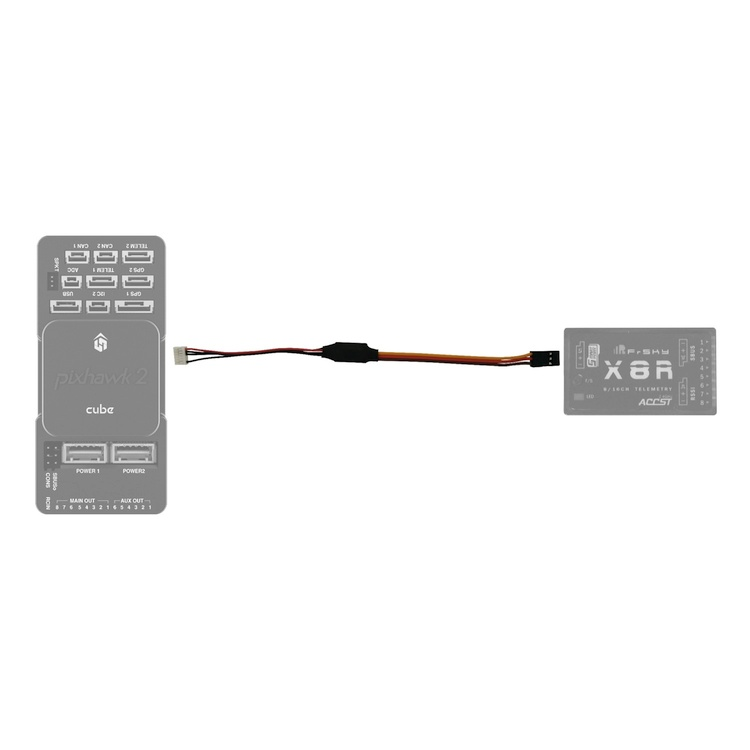
\includegraphics[width=\linewidth]{img/frsky-x8r.jpg}\\{\small Приёмник FrSky и полётный контроллер}\end{minipage}\hspace{1cm}
\begin{minipage}[b]{0.34\linewidth}\centering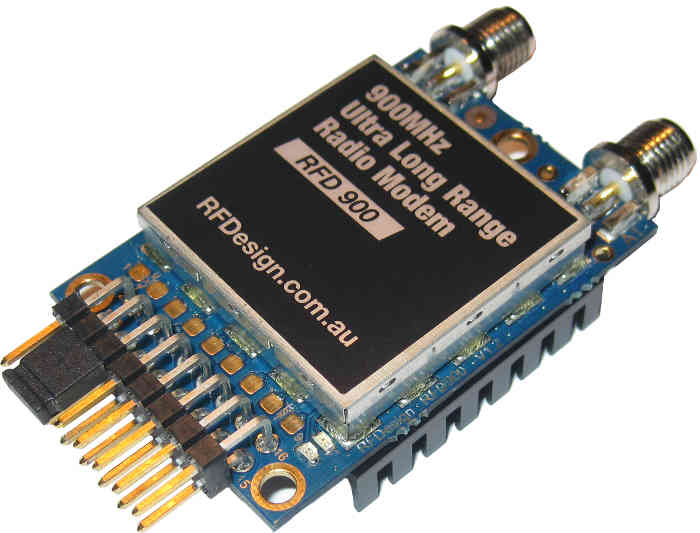
\includegraphics[width=\linewidth]{img/rfd900.jpg}\\{\small Модем телеметрии RFD900}\end{minipage}
\caption{Приёмник и модем телеметрии {\color{gray}\scriptsize(фото: ArduPilot Wiki)}}
\end{figure}

\subsection{Сравнение по частотам}
\begin{table}[H]\centering\small
\renewcommand{\arraystretch}{1.25}
\begin{tabularx}{\linewidth}{@{}p{25mm} X X@{}}
\toprule
 & \textbf{2,4 ГГц} & \textbf{868/915 МГц} \\
\midrule
Системы & ELRS 2.4, Tracer, FrSky ACCST/ACCESS, FlySky, Spektrum & ELRS 900, Crossfire, FrSky R9, mLRS \\
Задержка & меньше (до 1000 Гц) & больше (25–200 Гц) \\
Дальность & меньше & больше (меньше затухание) \\
Огибание препятствий & хуже & лучше (длиннее волна) \\
Антенны & маленькие (\SI{3}{\centi\metre}) & крупнее (\SI{8}{\centi\metre}, «T»-антенны) \\
Помехи & Wi-Fi, Bluetooth & меньше, но LoRa-устройства, GSM-900 \\
\bottomrule
\end{tabularx}
\caption{2,4 ГГц против 868/915 МГц}
\end{table}

\begin{caution}[Частоты и мощность в России]
Без разрешения можно использовать только устройства в разрешённых полосах и с ограниченной мощностью (решения ГКРЧ; для 868~МГц и 2,4~ГГц — единицы–сотни милливатт в зависимости от полосы). Мощные передатчики (1–2~Вт) и нестандартные частоты требуют разрешения. Диапазон 915~МГц (США) в России не выделен для таких устройств — используйте прошивку/регион \textbf{EU 868}.
\end{caution}

\begin{exam}
\begin{enumerate}
\item Почему ELRS вытеснил FrSky? Какие модуляции использует ELRS?
\item Как связаны частота пакетов, задержка и дальность?
\item Что такое failsafe, RSSI и LQ?
\item Чем 900-мегагерцовые системы лучше 2,4 ГГц и чем хуже?
\end{enumerate}
\end{exam}
